%%%%%%%%%%%%%%%%%%%%%%%%%%%%%%%%%%%%%%%%%%%%%%%%%%%%%%%%%%%%%%%%%%%%%%%%%%%%%%
% Trabalho Java RMI de Desenvolvimento de Aplicações Móveis e Distribuídas
%%%%%%%%%%%%%%%%%%%%%%%%%%%%%%%%%%%%%%%%%%%%%%%%%%%%%%%%%%%%%%%%%%%%%%%%%%%%%%
\documentclass[12pt,brazil, a4paper, fullpage]{article}

%%%%%%%%%%%%%%%%%%%%%%%%%%%%%%%%%%%%%%%%%%%%%%%%%%%%%%%%%%%%%%%%%%%%%%%%%%%%%%
% Preambulo - Configuração de página
%%%%%%%%%%%%%%%%%%%%%%%%%%%%%%%%%%%%%%%%%%%%%%%%%%%%%%%%%%%%%%%%%%%%%%%%%%%%%%
%%%%%%%%%%%%%%%%%%%%%%%%%%%%%%%%%%%%%%%%%%%%%%%%%%%%%%%%%%%%%%%%%%%%%%%%%%%%%%
% Preambulo - Pacotes
%%%%%%%%%%%%%%%%%%%%%%%%%%%%%%%%%%%%%%%%%%%%%%%%%%%%%%%%%%%%%%%%%%%%%%%%%%%%%%
\usepackage[table]{xcolor}
\usepackage{geometry}
\usepackage[portuges]{babel}
\usepackage[portuges]{translator}
\usepackage[T1]{fontenc}
\usepackage[utf8]{inputenc}
\usepackage{epsfig}
\usepackage{multirow}
\usepackage{tikz}
\usepackage{listings}
\usepackage{natbib}
\usepackage{hyperref}
\usepackage{multicol}
\usepackage{fancyhdr}
\usepackage{enumitem}

%%%%%%%%%%%%%%%%%%%%%%%%%%%%%%%%%%%%%%%%%%%%%%%%%%%%%%%%%%%%%%%%%%%%%%%%%%%%%%
% Preambulo - Configuração de Página
%%%%%%%%%%%%%%%%%%%%%%%%%%%%%%%%%%%%%%%%%%%%%%%%%%%%%%%%%%%%%%%%%%%%%%%%%%%%%%
\setlength{\topmargin}{0pt}
\setlength{\voffset}{-1.8cm}
\setlength{\textheight}{25,6cm}
\setlength{\oddsidemargin}{0cm}
\setlength{\evensidemargin}{0cm}
\setlength{\hoffset}{-1cm}
\setlength{\textwidth}{18cm}

\pagestyle{empty}

\input xy
\xyoption{all}
\xyoption{color}



%%%%%%%%%%%%%%%%%%%%%%%%%%%%%%%%%%%%%%%%%%%%%%%%%%%%%%%%%%%%%%%%%%%%%%%%%%%%%%
% Define cabeçalho de prova
%%%%%%%%%%%%%%%%%%%%%%%%%%%%%%%%%%%%%%%%%%%%%%%%%%%%%%%%%%%%%%%%%%%%%%%%%%%%%%
\newcommand{\cabecalhoProva}{
\pagestyle{fancy} % define página com cabeçalho
\fancyhf{} % limpa todos os cabeçalhos e rodapés
\setlength{\headheight}{22pt} %% define tamanho personalizado de cabeçalho
\renewcommand{\headrulewidth}{0pt} % elimina a linha de separação do cabeçalho
\fancyhead[LO]{\dadosAluno}
}


%%%%%%%%%%%%%%%%%%%%%%%%%%%%%%%%%%%%%%%%%%%%%%%%%%%%%%%%%%%%%%%%%%%%%%%%%%%%%%
% Logo da PUC Minas
%%%%%%%%%%%%%%%%%%%%%%%%%%%%%%%%%%%%%%%%%%%%%%%%%%%%%%%%%%%%%%%%%%%%%%%%%%%%%%
\newcommand{\logoPUC}[2]{
\begin{center}\renewcommand{\tabcolsep}{3mm}
    \begin{tabular*}{\textwidth}{ll}
        \multirow{4}{*}{\includegraphics[height=1.4cm]{#2}}
        &   \\
        & \usefont{T1}{cmss}{bx}{n} PONTIFÍCIA  UNIVERSIDADE  CATÓLICA  DE  MINAS  GERAIS  \\
        &  \usefont{T1}{cmss}{bx}{n} #1\vspace{2mm}\\
        &   \\
    \end{tabular*}
\end{center}
}

%%%%%%%%%%%%%%%%%%%%%%%%%%%%%%%%%%%%%%%%%%%%%%%%%%%%%%%%%%%%%%%%%%%%%%%%%%%%%%
% Caracteristicas da disciplina
%%%%%%%%%%%%%%%%%%%%%%%%%%%%%%%%%%%%%%%%%%%%%%%%%%%%%%%%%%%%%%%%%%%%%%%%%%%%%%

\newcommand{\dadosDisciplina}[5]{
\begin{center}
\begin{tabular*}{\textwidth}{|p{7.5cm}@{\extracolsep{\fill}}|p{5.5cm}|p{2cm}|p{1.2cm}|}
    \hline
    \sf Disciplina & \sf Departamento & \sf Turno & \sf Período \\
    
    \multicolumn{1}{|c|}{#1} &
    \multicolumn{1}{c|}{#2} &
    \multicolumn{1}{c|}{#3} &
    \multicolumn{1}{r|}{#4$^\circ$} \\ \hline \hline
    \multicolumn{4}{|l|}{\sf Professor} \\
    \multicolumn{4}{|l|}{\hspace{1cm} #5} \\ \hline
\end{tabular*}
\end{center}
}


\newcommand{\dadosAluno}{
\begin{tabular*}{\textwidth}{|p{.2\textwidth}@{\extracolsep{\fill}}|p{.75\textwidth}|}
	\hline
	\sf Matrícula: & \sf Aluno: \\
	\hspace{1cm} & \hspace{1cm} \\
	\hline
\end{tabular*}
}


%%%%%%%%%%%%%%%%%%%%%%%%%%%%%%%%%%%%%%%%%%%%%%%%%%%%%%%%%%%%%%%%%%%%%%%%%%%%%%
% Título simples
%%%%%%%%%%%%%%%%%%%%%%%%%%%%%%%%%%%%%%%%%%%%%%%%%%%%%%%%%%%%%%%%%%%%%%%%%%%%%%
\newcommand{\tituloPUC}[1]{
\vspace{3mm}

\begin{center}
    {\Large \bf #1}
\end{center}

\vspace{3mm}
}



%%%%%%%%%%%%%%%%%%%%%%%%%%%%%%%%%%%%%%%%%%%%%%%%%%%%%%%%%%%%%%%%%%%%%%%%%%%%%%
% Comandos para gabarito
%%%%%%%%%%%%%%%%%%%%%%%%%%%%%%%%%%%%%%%%%%%%%%%%%%%%%%%%%%%%%%%%%%%%%%%%%%%%%%
\newcommand{\itemvf}[1]{\item ( \ifgabarito  #1 \else\hspace{8mm}\fi )}
\newcommand{\itemresp}[1]{\ifgabarito \textbf{\item #1} \else \item #1 \fi}


\usepackage{booktabs}
\usepackage{wrapfig}


%%%%%%%%%%%%%%%%%%%%%%%%%%%%%%%%%%%%%%%%%%%%%%%%%%%%%%%%%%%%%%%%%%%%%%%%%%%%%%
% Inicio do documento
%%%%%%%%%%%%%%%%%%%%%%%%%%%%%%%%%%%%%%%%%%%%%%%%%%%%%%%%%%%%%%%%%%%%%%%%%%%%%%
\begin{document}

    \selectlanguage{brazil}
    \lstset{language=Java,
        basicstyle=\small, % print whole listing small
        showstringspaces=false}

%%%%%%%%%%%%%%%%%%%%%%%%%%%%%%%%%%%%%%%%%%%%%%%%%%%%%%%%%%%%%%%%%%%%%%%%%%%%%%
% Logo da PUC Minas
%%%%%%%%%%%%%%%%%%%%%%%%%%%%%%%%%%%%%%%%%%%%%%%%%%%%%%%%%%%%%%%%%%%%%%%%%%%%%%
\thispagestyle{plain}
\logoPUC{Curso de Bacharelado em Engenharia de Software}{puc_engesoft_logo.png}

%%%%%%%%%%%%%%%%%%%%%%%%%%%%%%%%%%%%%%%%%%%%%%%%%%%%%%%%%%%%%%%%%%%%%%%%%%%%%%
% Caracteristicas da disciplina
%%%%%%%%%%%%%%%%%%%%%%%%%%%%%%%%%%%%%%%%%%%%%%%%%%%%%%%%%%%%%%%%%%%%%%%%%%%%%%
\dadosDisciplina{Lab. Desenv. Aplic. Móveis e Distribuás}{Engenharia de Software}{Noite}{5}{Hugo de Paula (hugo@pucminas.br)}

\tituloPUC{Trabalho Bolsa de Valores \\ em dupla}


%%%%%%%%%%%%%%%%%%%%%%%%%%%%%%%%%%%%%%%%%%%%%%%%%%%%%%%%%%%%%%%%%%%%%%%%%%%%%%
% Corpo
%%%%%%%%%%%%%%%%%%%%%%%%%%%%%%%%%%%%%%%%%%%%%%%%%%%%%%%%%%%%%%%%%%%%%%%%%%%%%%

\section{Introdução}

Middlewares orientados a mensagens (MOM – \textit{Message Oriented Middlewares}) são sistemas que permitem o envio de mensagens entre entidades de um sistema distribuído. São uma forma de comunicação indireta que provê um serviço de comunicação baseado em filas de mensagens, promovendo o desacoplamento de tempo e espaço. A Seção 6.4 da 5a edição do livro Distributed Systems, do Coulouris (2013), descreve o modelo de programação de MOM.

O \textit{Java Message Service} – JMS e o \textit{Advanced Message Queueing Protocol} – AMQP são APIs que especificam modelos de middleware orientado a mensagens. Esses middlewares suportam pelo menos dois modelos básicos de troca de mensagens: ponto a ponto e o modelo \textit{publish/subscribe}. Para que uma aplicação possa utilizar o middleware, deve haver um provedor que possa gerenciar as sessões e filas. Existem opções comerciais e livres de sistemas MOM. Dentre as opções FOSS tem-se: ActiveMQ, JBossMQ, HornetQ, Joram, MantaRay, OpenJMS, RabbitMQ.



\section{Objetivos do trabalho}

Neste trabalho deverá ser desenvolvido um sistema para uma bolsa de valores qualquer, como a Bovespa, utilizando o RabbitMQ. Quem quiser conhecer um pouco mais sobre o funcionamento da bolsa de valores, visite o site da BOVESPA em \url{http://www.b3.com.br/pt_br/market-data-e-indices/servicos-de-dados/market-data/cotacoes/}.


\section{Especificação}

\indent \indent A corretora (ou broker) pode enviar as seguintes operações à bolsa de valores:


\begin{tabular}{lcp{7.3cm}}
    \toprule
    \multicolumn{3}{c}{\textbf{Mensagens da Corretora → Bolsa de valores}} \\
    \midrule
    \textbf{OPER.} & \textbf{FORMATO DA MENSAGEM} & \textbf{DESCRIÇÃO} \\
    \midrule
    compra & <quant: int, val: real, corretora: char[4]> & Envia à bolsa de valores uma ordem de compra com o tópico compra.ativo indicando que a corretora deseja comprar quant lotes de ações de um ativo pelo preço de val reais. \\
    venda & <quant: int, val: real, corretora: char[4]> & Envia à bolsa de valores uma ordem de venda com o tópico venda.ativo indicando que a corretora deseja vender quant lotes de ações de um ativo pelo preço de val reais. \\
    \bottomrule
\end{tabular}%


\begin{tabular}{lcp{7.3cm}}
    \toprule
    \multicolumn{3}{c}{\textbf{Mensagens da Bolsa de valores → Corretora}} \\
    \midrule
    \textbf{OPER.} & \textbf{FORMATO DA MENSAGEM} & \textbf{DESCRIÇÃO} \\
    \midrule
    compra & <quant: int, val: real, corretora: char[4]> & Envia ao tópico compra.ativo uma mensagem notificando que a bolsa de valores recebeu uma ordem de compra. \\
    venda & <quant: int, val: real, corretora: char[4]> & Envia ao tópico venda.ativo uma mensagem notificando que a bolsa de valores recebeu uma ordem de compra. \\
    \bottomrule
\end{tabular}%


O diagrama de sequência a seguir ilustra um cenário de troca de mensagens entre uma Corretora e a Bolsa de valores. Linhas contínuas representam mensagens enviadas na estrutura de tópicos da Corretora para a Bolsa de Valores, enquanto as linhas tracejadas representam as mensagens enviadas da Bolsa de valores para as corretoras. \\

\begin{center}
    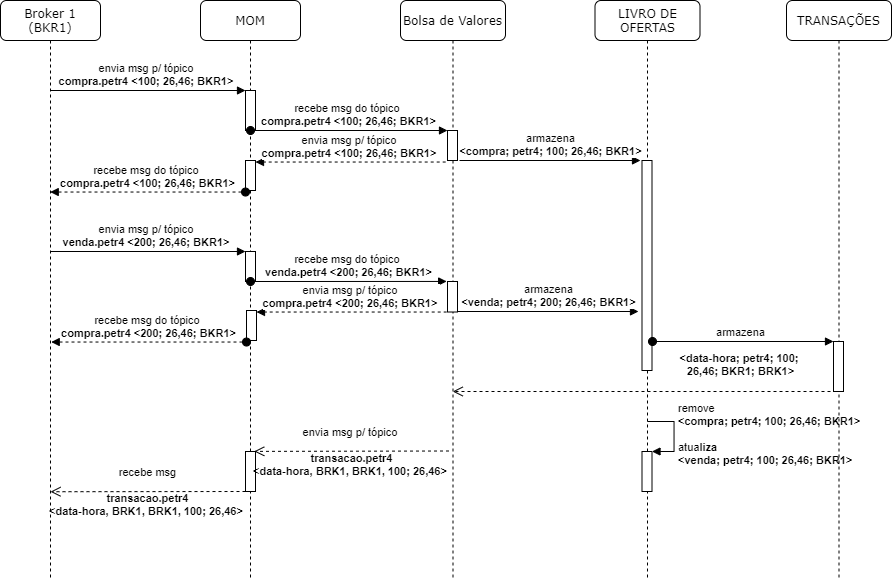
\includegraphics[width=.93\textwidth]{bolsadevalores.png} \\
\end{center}

As regras de negócio do sistema podem ser descritas da seguinte forma:

\begin{itemize}
    \item Brokers podem enviar ORDENS DE COMPRA, ORDENS DE VENDA para a bolsa de valores.
    \item Brokers podem assinar tópicos relativos aos ativos que desejam acompanhar.
    \item Sempre que a bolsa de valores recebe uma ordem de compra ou de venda, ela deve encaminhar essa ordem a todos os brokers os interessados naquela ação específica através de um mecanismo de tópicos.
    \item Sempre que o valor de uma ORDEM DE COMPRA for maior ou igual ao valor de uma ORDEM DE VENDA para um mesmo ativo, a bolsa de valores deve gerar uma mensagem do tipo TRANSAÇÃO no tópico adequado, e atualizar/remover as ordens da fila.
    \item Os brokers deverão encaminhar mensagens para uma
    \item A bolsa de valores e os brokers deverão usar uma estrutura de tópicos, do tipo: operacao.ativo.
\end{itemize}

O sistema deve ser carregado com a lista de ativos da Bovespa. A tabela a seguir ilustra alguns exemplos de ativos da Bovespa.

% Table generated by Excel2LaTeX from sheet 'Planilha2'
\begin{tabular}{llp{10cm}}
    \toprule
    \multicolumn{3}{c}{\textbf{Lista de ativos resumida}}  \\
    \midrule
    \textbf{NOME DE PREGÃO} & \textbf{CÓDIGO} & \textbf{ATIVIDADE PRINCIPAL} \\
    AMBEV S/A ON & ABEV3 & Fabricação e Distribuição de Cervejas. Refrigerantes e Bebidas não Carbonatadas e não Alcoólicas. \\
    PETROBRAS PN & PETR4 & Petróleo. Gás e Energia \\
    VALE PNA & VALE5 & Mineração \\
    ITAU UNiBANCO PN & ITUB4 & A Sociedade Tem por Objeto A Atividade Bancária. \\
    BRADESCO PN & BBDC4 & Prática de Operações Bancárias em Geral. inclusive Câmbio \\
    BRASIL ON & BBAS3 & Banco Múltiplo. \\
    CIELO ON & CIEL3 & Empresa Prestadora de Serviços de Adquirência e Meios de Pagamento \\
    PETROBRAS ON & PETR3 & Petróleo. Gás e Energia. \\
    HYPERMARCAS ON & HYPE3 & Produção e Venda de Bens de Consumo e Medicamentos. \\
    VALE ON & VALE3 & Mineração \\
    BBSEGURIDADE ON & BBSE3 & Participação no Capital Social de Outras Sociedades. que Tenham por Atividade Operações de Seguros. Resseguros. Previdências Complementar ou Capitaliüação. \\
    CETIP ON & CTIP3 & Sociedade Administradora de Mercados de Balcão Organiüados. \\
    GERDAU PN & GGBR4 & Participação e Administração. \\
    FIBRIA ON & FIBR3 &  \\
    RAIADROGASIL ON & RADL3 & Comércio de Produtos Farmacêuticos. Perfumarias e Afins. \\
    \bottomrule
\end{tabular}%

\section{Atividades}

Inicialmente, o grupo deverá:
\begin{enumerate}
    \item 	Instalar o RabbitMQ, disponível em https://www.rabbitmq.com
    \item 	Executar os tutoriais l a 5.
\end{enumerate}

O trabalho consiste em desenvolver um pequeno aplicativo para o Broker e outro aplicativo para a Bolsa de valores, utilizando filas de mensagens e estruturas de tópicos. Os requisitos do trabalho são:

\begin{enumerate}
    \item O servidor do RabbitMQ deve ser configurado na nuvem no site \url{https://www.cloudamqp.com/}.
    Crie uma máquina gratuita do tipo \textit{Little Lemur - For Development}.
    \item O endereço do RabbitMQ server deve ser passado como parâmetro para que brokers e bolsas possam escolher a quem se conectar.
    \item A bolsa deve abrir um canal do tipo pub/sub utilizando tópicos para publicar as atualizações no livro de ofertas e as operações realizadas em uma ação. O nome do canal deve ser BOLSADEVALORES.
    \item O servidor abre uma fila de mensagens para receber as operações dos clientes. O nome da fila de mensagens deve ser BROKER.
    \item Os clientes enviam operações para o servidor através da fila de mensagens BROKER.
    \item Todos os clientes devem receber a notificação das operações através da fila BOLSADEVALORES.
    \item O servidor deverá ser disponibilizado em uma máquina diferente de localhost.
    \item O aplicativo deve funcionar nas máquinas Linux do laboratório de redes do curso de Engenharia de Software da PUC Minas.
\end{enumerate}

Observações:
\begin{enumerate}
    \item Será necessário utilizar Threads em Java.
    \item O Tutorial 1 do RabbitMQ ensina como criar o canal para o recebimento da mensagem pelo servidor.
    \item O Tutorial 3 do RabbitMQ ensina como criar a exchange box para o Publish/Subscribe.
    \item O Tutorial 5 do RabbitMQ ensina como utilizar uma estrutura de tópicos.
\end{enumerate}


\section{Resultados Esperados}

Deverá ser entregue:

\begin{enumerate}
    \item Todo o código, comentado.

    \item Um arquivo README.TXT contendo uma explicação sucinta do código e instruções para compilação e execução do mesmo.
\end{enumerate}


\end{document}
